\documentclass[sigconf]{acmart}

\usepackage{graphicx}
\usepackage{amsmath}
\usepackage{enumitem}
\usepackage{booktabs}
\usepackage{placeins}
\usepackage{subcaption}

\settopmatter{printacmref=false}
\renewcommand\footnotetextcopyrightpermission[1]{}
\pagestyle{plain}

\acmConference[ICAIF '26]{ACM ICAIF}{2026}{New York, USA}

\begin{CCSXML}
<ccs2012>
   <concept>
       <concept_id>10010147.10010178.10010187</concept_id>
       <concept_desc>Computing methodologies~Reinforcement learning</concept_desc>
       <concept_significance>500</concept_significance>
   </concept>
   <concept>
       <concept_id>10010405.10010455.10010458</concept_id>
       <concept_desc>Applied computing~Economics</concept_desc>
       <concept_significance>300</concept_significance>
   </concept>
   <concept>
       <concept_id>10010147.10010257.10010293.10010294</concept_id>
       <concept_desc>Computing methodologies~Multi-agent systems</concept_desc>
       <concept_significance>300</concept_significance>
   </concept>
</ccs2012>
\end{CCSXML}

\ccsdesc[500]{Computing methodologies~Reinforcement learning}
\ccsdesc[300]{Applied computing~Economics}
\ccsdesc[300]{Computing methodologies~Multi-agent systems}

\keywords{reinforcement learning, market microstructure, agent-based simulation, limit order book, liquidity, multi-agent systems}

\title{Persistent One-Sided Order Books from Learned Trading Behavior}
\author{Jean-Paul Vestjens \\ \texttt{vestjejj@rose-hulman.edu}}
\date{}

\begin{document}

\begin{abstract}
We study how increasing the fraction $\phi$ of reinforcement learning (RL) trading agents in an agent-based market simulation affects limit order book liquidity. As $\phi$ rises above a predicted threshold $\phi^* \approx 0.26$, persistent one-sided order book states emerge — where either the best bid or best ask disappears and the mid-price becomes undefined. A matched-composition control shows that both trained and random replacement agents produce severe failures above the threshold, confirming the effect is a structural property of RL participation fraction rather than an artifact of learned policy coordination. Inventory constraints substantially reduce both the frequency and persistence of these failures, identifying a practical structural mitigation.
\end{abstract}

\maketitle
\hypersetup{hidelinks}

\section{Introduction}

Financial markets require continuous two-sided liquidity: both buy and sell orders must be present for prices to form through matching. When one side of the limit order book disappears, mid-price formation breaks down and spreads become undefined. Understanding how such failures emerge is a central problem in market microstructure.

This paper shows that, in simulation, increasing the participation of RL agents — parameterized by $\phi$ — produces a nonlinear rise in persistent one-sided order book states. Prior work on RL in financial markets has optimized individual execution and market-making performance \cite{spooner2018,nevmyvaka2006}, often via historical replay with negligible market impact \cite{balch2019}. Agent-based studies have shown herding and coordination effects can reduce matching and liquidity \cite{lussange2024}, and policy-oriented work has highlighted that algorithmic trading may withdraw liquidity under stress \cite{farmer2009,boe2018,imf2023}. The present work differs in three ways: the dependent variable is top-of-book structure (whether the best bid or ask is present), RL participation is varied systematically across $\phi$ values, and the failure mode emerges from policies trained within a discrete-event limit order book framework \cite{byrd2020} rather than imitative strategies.

The specific contributions are: (1) empirical evidence that RL participation fraction $\phi$ produces a nonlinear threshold-like rise in persistent one-sided order book states; (2) an analytical flow-rate model predicting $\phi^* \approx 0.26$ that aligns with the empirical transition; (3) a matched-composition control showing both trained and random replacement agents produce severe failures above the threshold, confirming the effect is structural; and (4) evidence that inventory constraints are an effective structural mitigation.

\section{Methods}

\subsection{Market Environment and RL Participation}

All experiments use an ABIDES-based simulation \cite{byrd2020} with a frozen RMSC-style configuration of 102 agents interacting through a central exchange driven by a Gaussian random-walk oracle. The baseline ($\phi=0$) population consists of 80 noise traders (the primary source of passive liquidity), 20 value traders, and 2 adaptive market makers. The primary control parameter $\phi$ replaces a fraction of the 80 noise traders with RL agents, keeping value traders and market makers fixed:
\[
\phi \in \{0.00,\; 0.05,\; 0.10,\; 0.20,\; 0.30,\; 0.40,\; 0.50\}.
\]

\subsection{RL Liquidity Provision Modes}

All primary experiments use the \textbf{taker-only} configuration: RL agents choose among buy market order, sell market order, or hold. No limit orders are submitted, so RL agents act exclusively as liquidity consumers. This is the cleanest setting for isolating one-sided failure: every RL action that executes removes volume from one side of the book.

\subsection{RL Agent Design}

Each taker agent has a discrete action space \{sell, hold, buy\} producing market orders of size 1. The quoting agent action space additionally includes limit-quote actions. The state vector is 13-dimensional: a rolling window of 10 log returns, bid-ask spread, order-book imbalance, and current inventory.

Rewards per decision step are:
\begin{equation}
r_t = \Delta W_t - \lambda_q \cdot 100 \cdot q_t^2 - P_{\text{hold}} - P_{\text{anti-deg}}
\label{eq:reward}
\end{equation}
where $\Delta W_t$ is the marked-to-market wealth change, $q_t$ is inventory ($\lambda_q = 0.01$), $P_{\text{hold}}$ is a flat penalty applied when the agent holds with zero inventory, and $P_{\text{anti-deg}}$ is an escalating hold-streak penalty that activates after a configurable grace period of consecutive hold actions to discourage prolonged inactivity. In quoting configurations, additional terms reward passive fills and penalize missing two-sided quotes; these terms are zero in taker-only experiments.

When inventory constraints are enabled, actions that would violate a hard cap are silently converted to hold.

Agents are trained with PPO using Generalized Advantage Estimation. The policy is a single linear softmax layer (no hidden layers) mapping the 13-dimensional state to action logits; a separate linear value head estimates returns. All agents at a given $\phi$ share one policy object; a fresh policy is trained per $\phi$ value. Table~\ref{tab:hyperparams} lists training hyperparameters.

\begin{table}[htbp]
\caption{PPO training hyperparameters.}
\label{tab:hyperparams}
\begin{tabular}{ll}
\toprule
Parameter & Value \\
\midrule
Optimizer & Adam \\
Actor / Critic LR & 0.01 / 0.02 \\
Discount $\gamma$ & 0.99 \\
GAE $\lambda$ & 0.95 \\
PPO clip $\varepsilon$ & 0.2 \\
Update epochs / rollout & 4 \\
Minibatch size & 256 \\
Entropy coefficient & 0.01 \\
Gradient clip norm & 1.0 \\
\bottomrule
\end{tabular}
\end{table}

\subsection{One-Sided Order Book Definition}

A timestep is classified as one-sided when exactly one side has positive visible volume while the other has zero: $(\text{bid\_vol} > 0) \oplus (\text{ask\_vol} > 0)$, evaluated only on timesteps with at least one non-zero side. When one-sided, the mid-price is undefined and the spread cannot be computed.

\subsection{Experiment Protocol}

Table~\ref{tab:protocol} summarizes the protocol. For each $\phi$, a policy is trained on 50 episodes; evaluation uses 6 seeds in both greedy and stochastic modes (12 runs per $\phi$). Confidence intervals are 95\% bootstrap CIs across evaluation runs.

\begin{table}[htbp]
\caption{Experiment protocol.}
\label{tab:protocol}
\begin{tabular}{@{}p{0.52\columnwidth}p{0.42\columnwidth}@{}}
\toprule
Parameter & Value \\
\midrule
Simulation horizon & 5 min (09:30--09:35) \\
Training episodes per $\phi$ & 50 \\
Evaluation seeds & 7--12 (6 seeds) \\
Evaluation modes & Greedy and stochastic \\
Eval.\ runs per $\phi$ & 12 \\
Policy reuse across $\phi$ & No \\
RL / noise wake freq.\ & 1 s / 5 s \\
RL order size & 1 unit \\
\bottomrule
\end{tabular}
\end{table}

\section{Results}

\subsection{Emergence and Persistence of One-Sided States}

As shown in Figure~\ref{fig:one-sided-book}, the fraction of one-sided timesteps remains below 4\% for $\phi \leq 0.20$ and spikes sharply at $\phi = 0.30$--$0.40$. This is not a gradual degradation but a threshold-like transition where liquidity consumption overwhelms replenishment.

\begin{figure}[htbp]
    \centering
    
\includegraphics[width=\columnwidth]{updated_one_sided_fraction.png}
    \caption{One-sided order book fraction vs.\ $\phi$ for greedy and stochastic evaluation. Error bars: 95\% bootstrap CIs over 12 evaluation runs.}
    \label{fig:one-sided-book}
\end{figure}

Figure~\ref{fig:duration} shows that once the system enters a one-sided state, recovery becomes increasingly difficult: both the maximum consecutive duration and the 90th-percentile episode duration rise sharply between $\phi = 0.30$ and $\phi = 0.40$. These failures are therefore not transient flickers but structurally persistent.

\begin{figure}[htbp]
    \centering
    \begin{subfigure}[b]{0.49\columnwidth}
        \centering
        
\includegraphics[width=\textwidth]{max_consecutive_one_sided_duration_with_ci_vs_phi.png}
        \caption{Max consecutive duration.}
        \label{fig:max-consecutive-duration}
    \end{subfigure}
    \hfill
    \begin{subfigure}[b]{0.49\columnwidth}
        \centering
        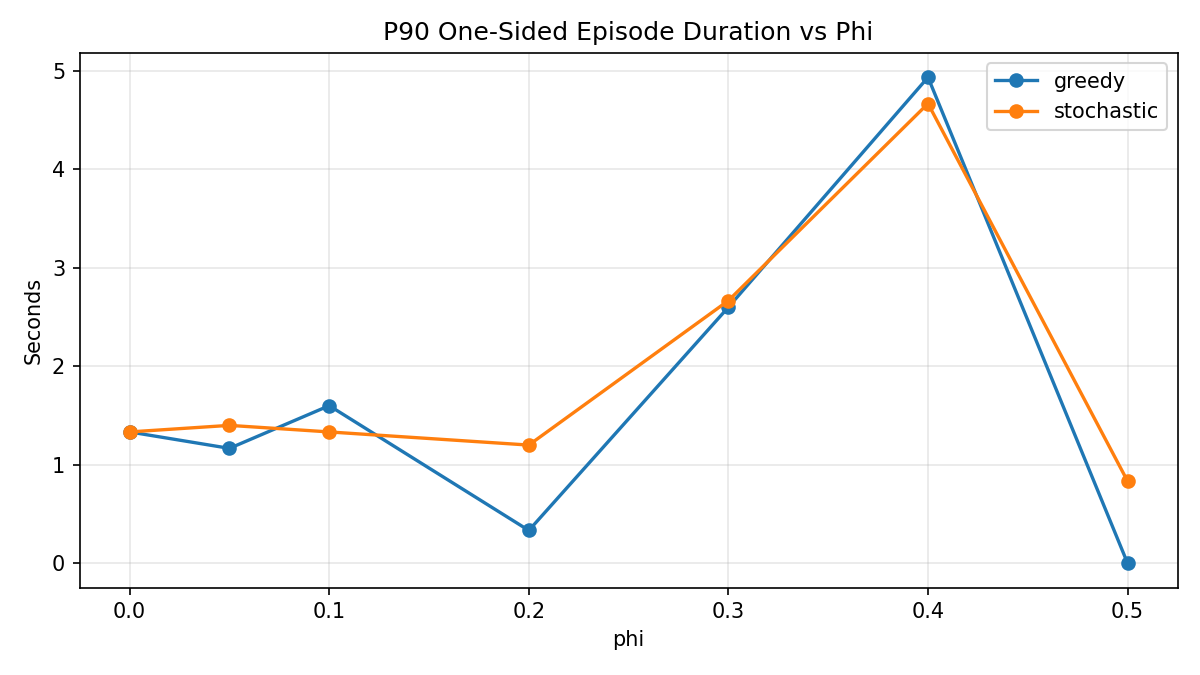
\includegraphics[width=\textwidth]{figure4.png}
        \caption{P90 episode duration.}
        \label{fig:p90-duration}
    \end{subfigure}
    \caption{Persistence of one-sided states. Both the maximum consecutive duration (left) and 90th-percentile episode length (right) spike sharply at $\phi = 0.30$--$0.40$.}
    \label{fig:duration}
\end{figure}

At $\phi = 0.5$ the one-sided fraction drops sharply, but this does not reflect improved liquidity. Figure~\ref{fig:shutdown-support} shows this coincides with near-total inactivity, collapsed quote activity, and a sharp rise in zero-return behavior — a degenerate market shutdown rather than recovery.

\begin{figure*}[htbp]
    \centering
    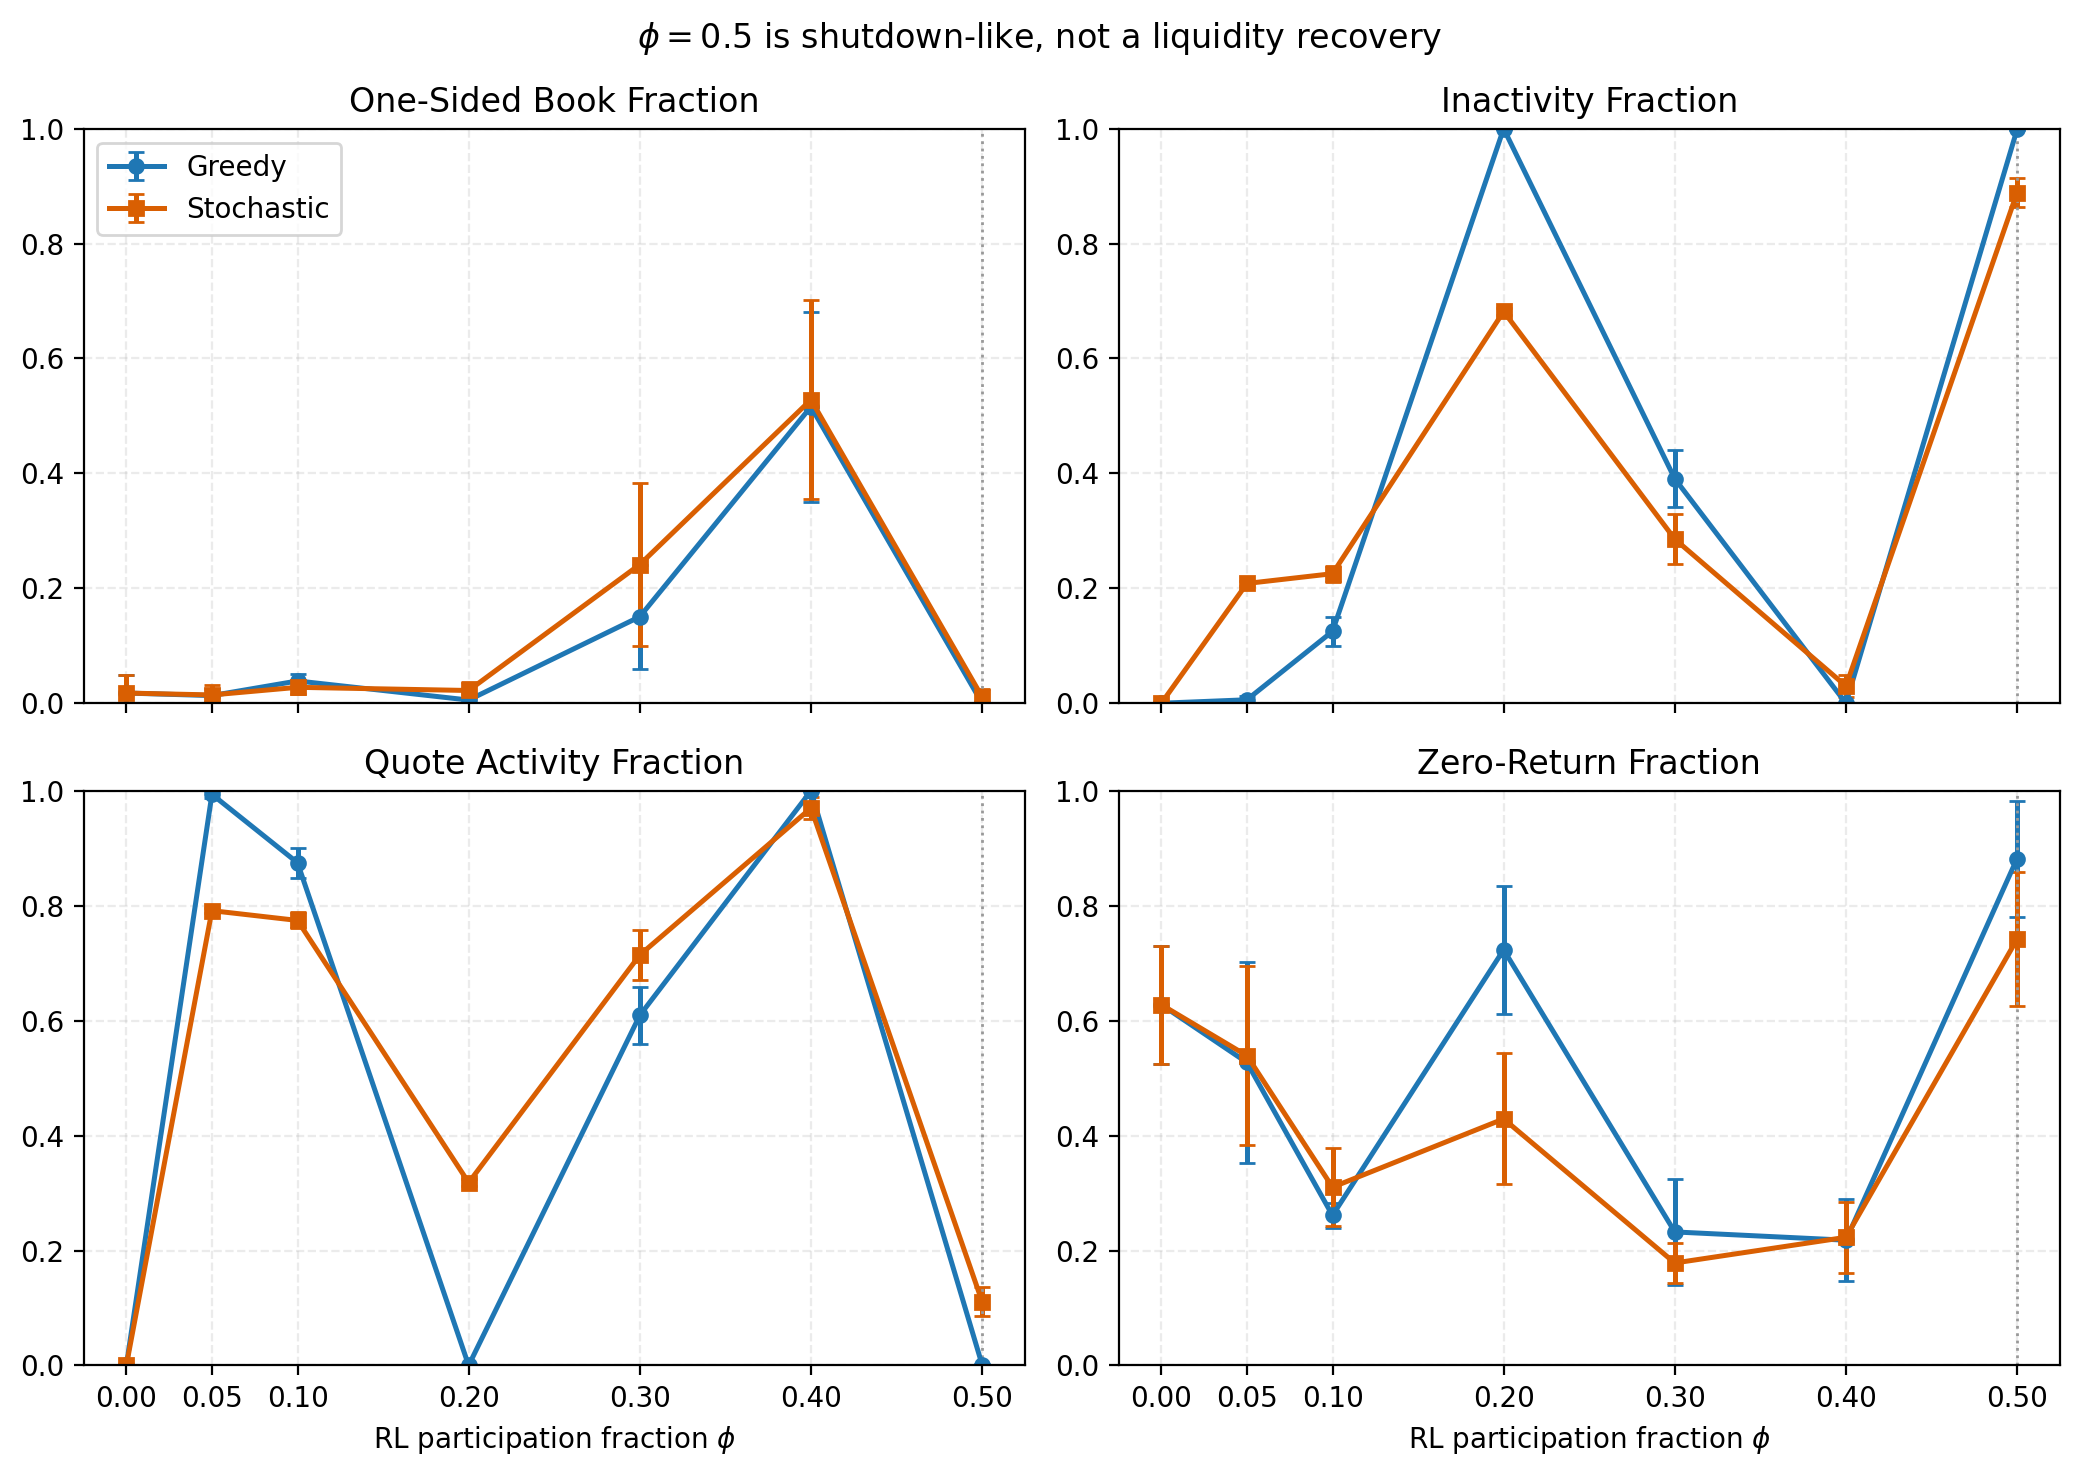
\includegraphics[width=\textwidth]{phi_0_5_shutdown_support.png}
    \caption{Evidence that $\phi = 0.5$ is a market shutdown rather than liquidity recovery. The drop in one-sided-book failures coincides with near-total inactivity, zero-return behavior, and collapsed quote activity.}
    \label{fig:shutdown-support}
\end{figure*}

\FloatBarrier

\subsection{Side-Specific Liquidity Failures}

Figure~\ref{fig:liquidity-modes} decomposes one-sided states into missing-bid and missing-ask failures. The missing-ask fraction dominates: as $\phi$ rises, RL agents predominantly issue buy market orders that consume ask-side liquidity, leaving the ask queue empty while the bid side remains intact. This directional asymmetry confirms that the failure is driven by the learned buy-biased execution strategy rather than symmetric noise in order flow.

\begin{figure*}[htbp]
    \centering
    
\includegraphics[width=\textwidth]{figure_both_test.png}
    \caption{Missing best-bid and missing best-ask fractions vs.\ $\phi$ (greedy and stochastic evaluation). The ask side fails predominantly, revealing a buy-bias in the learned policy that systematically depletes ask-side liquidity.}
    \label{fig:liquidity-modes}
\end{figure*}

\FloatBarrier

\subsection{Analytical Threshold}

The mechanism suggests a mean-field prediction. Let $C(\phi)$ and $P(\phi)$ denote aggregate liquidity consumption and provision:
\begin{align*}
C(\phi) &= 80\phi \cdot \lambda_r \\
P(\phi) &= 80(1-\phi) \cdot \lambda_n + 2\lambda_m
\end{align*}
where $\lambda_n = 0.09$ orders/s/noise trader (5 s wake, 0.45 submission probability) and $\lambda_m = 10$ units/s/market maker (1 s wake, size 5, both sides) follow directly from simulation parameters. Estimating $\lambda_r$ from low-$\phi$ pre-breakdown regimes gives $\lambda_r = 1.261$ at $\phi = 0.05$ and $\lambda_r = 1.209$ at $\phi = 0.10$, with mean $\bar{\lambda}_r = 1.235$ orders/s/agent.% TODO: update lambda_r from regen_headline_taker/summaries/per_seed_rl_diagnostics.csv

Setting $C(\phi^*) = P(\phi^*)$:
\[
\phi^* = \frac{80\lambda_n + 2\lambda_m}{80(\lambda_n + \lambda_r)} = 0.257 \quad [0.252,\; 0.262]% TODO: update phi* from threshold_analysis.py
\]

As shown in Figure~\ref{fig:threshold}, this prediction aligns with the empirical transition: one-sided failures remain below 4\% for $\phi \leq 0.20$ and spike sharply at $\phi = 0.30$, where excess consumption turns positive at $+4.61$ units/s. At $\phi = 0.40$, excess is $+15.21$ units/s (${\approx}63\%$), consistent with near-total one-sided failure.% TODO: update excess values from threshold_analysis.py

\begin{figure*}[htbp]
    \centering
    
\includegraphics[width=\textwidth]{threshold_analysis.png}
    \caption{Analytical threshold $\phi^*$ vs.\ empirical one-sided fraction. Left: flow rates cross at $\phi^* = 0.257$ (shaded band: uncertainty from $\lambda_r$ estimates). Right: empirical failure rate with predicted threshold overlaid; the sharp rise aligns with the crossing point.}
    \label{fig:threshold}
\end{figure*}

\FloatBarrier

\subsection{Effects of Inventory Constraints}

Figure~\ref{fig:inventory-cap-frequency} shows that inventory constraints significantly reduce one-sided state frequency across all $\phi$ values. Duration is also shortened (Figure~\ref{fig:inventory-cap-duration}). When agents cannot accumulate large directional positions, their ability to drain one side of the book is curtailed, and the system becomes meaningfully more stable — consistent with classical inventory-control models of market making \cite{avellaneda2008}.

\begin{figure}[htbp]
    \centering
    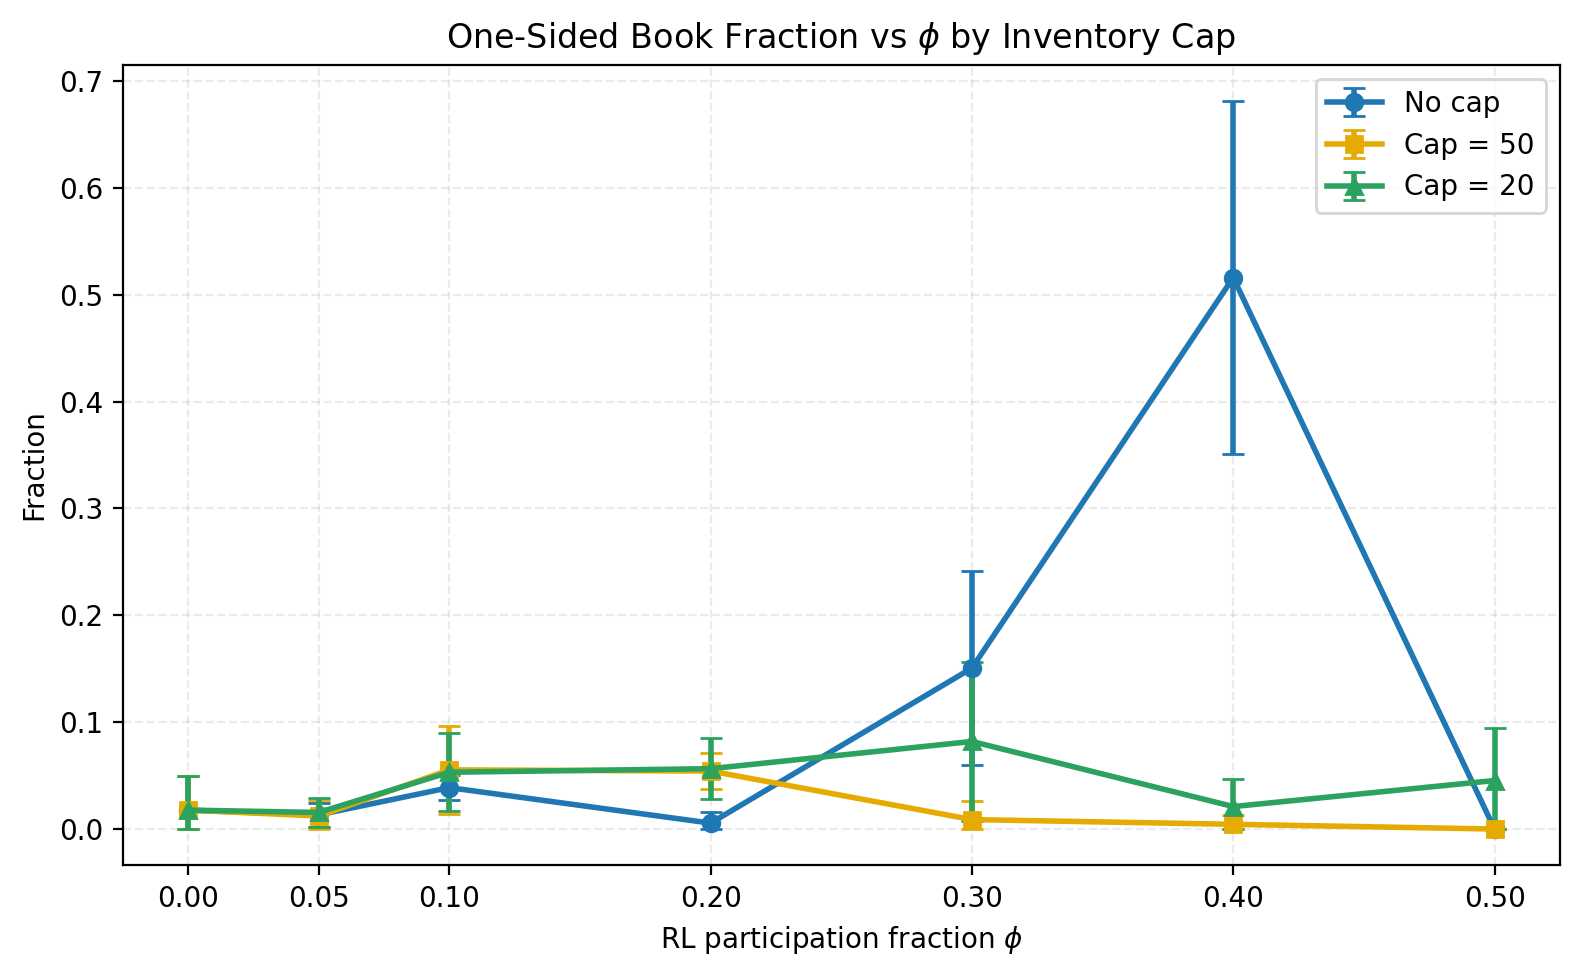
\includegraphics[width=\columnwidth]{inventory_cap_one_sided_fraction_with_ci_vs_phi.png}
    \caption{One-sided book fraction vs.\ $\phi$ by inventory cap. Constraints substantially reduce failure frequency.}
    \label{fig:inventory-cap-frequency}
\end{figure}

\begin{figure}[htbp]
    \centering
    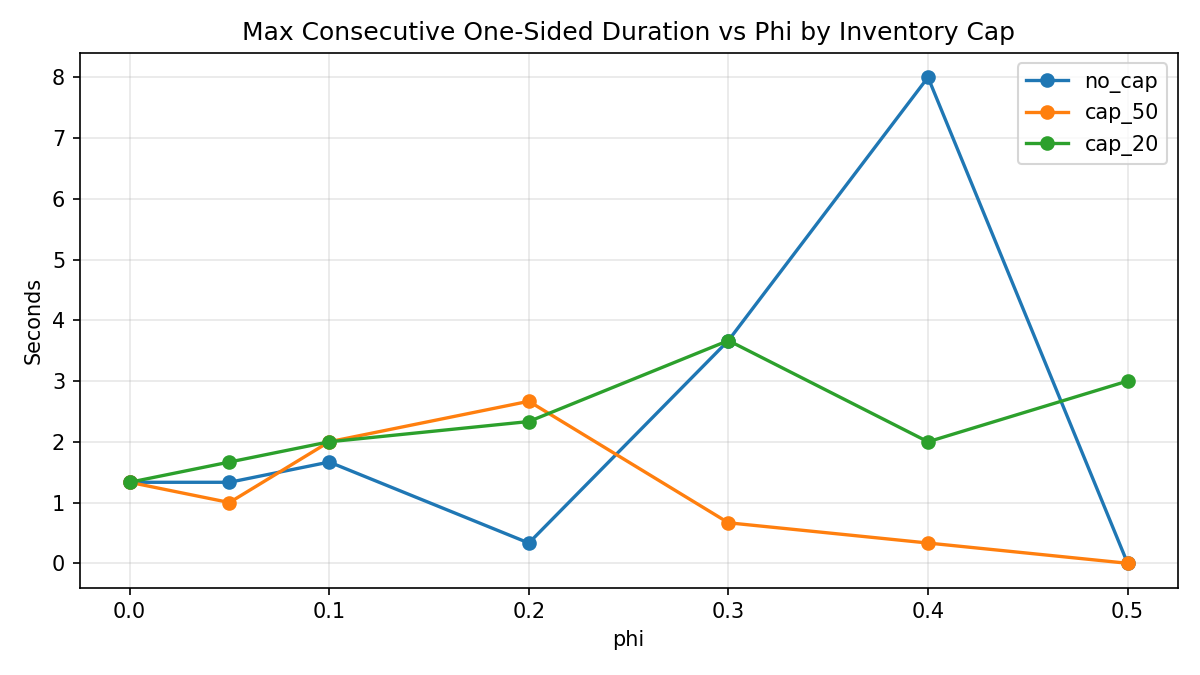
\includegraphics[width=\columnwidth]{figure10.png}
    \caption{Maximum consecutive one-sided duration vs.\ $\phi$ by inventory cap.}
    \label{fig:inventory-cap-duration}
\end{figure}

\FloatBarrier

\subsection{Trained Policies vs.\ Random Baseline}

Figure~\ref{fig:policy-type} compares trained RL agents with matched-composition random-policy agents (same $\phi$, uniformly random buy/hold/sell). At $\phi = 0.40$, the trained policy reaches $30.6\%$ (95\% CI $[21.7\%,\;41.4\%]$) and the random baseline reaches $26.3\%$ (95\% CI $[18.1\%,\;36.2\%]$); the CIs overlap substantially, indicating no statistically reliable difference at this $\phi$ level. Both conditions produce severe one-sided failures well above the baseline ($<1\%$ at $\phi=0$), confirming that the threshold effect is a structural property of RL participation fraction rather than an artifact of learned policy coordination. At $\phi = 0.30$, the random baseline ($16.5\%$) is numerically higher than the trained policy ($8.3\%$), consistent with trained agents having partially learned inventory management that delays onset; this advantage disappears above the threshold.

\begin{figure}[htbp]
    \centering
    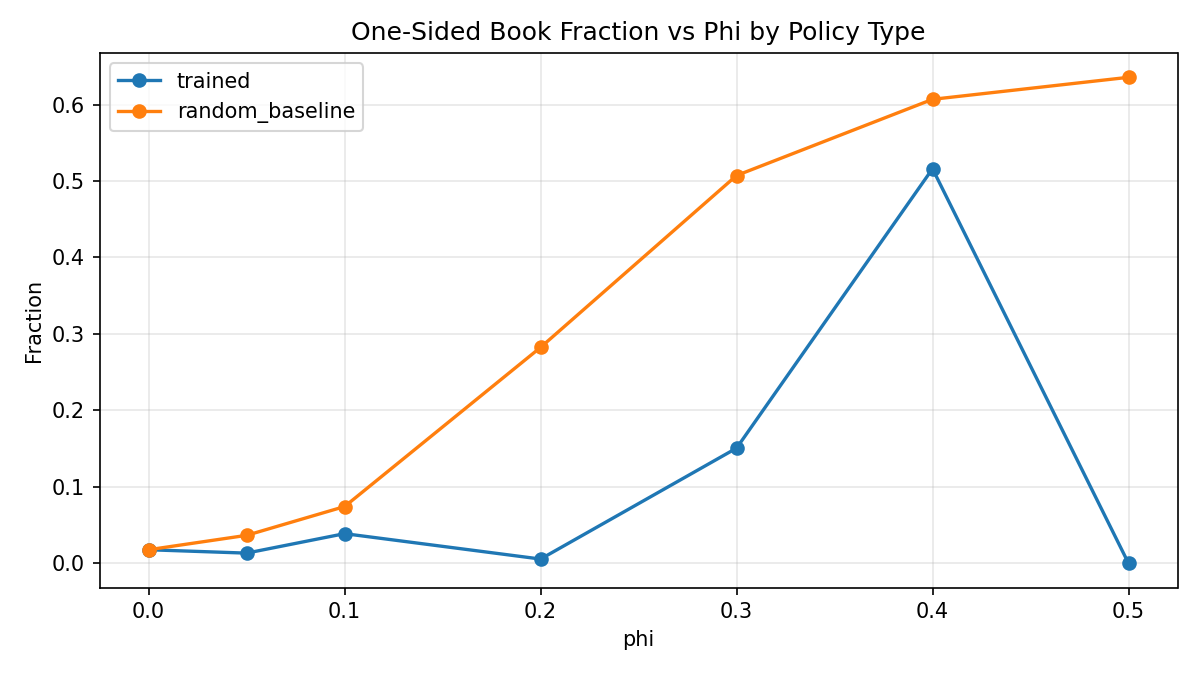
\includegraphics[width=\columnwidth]{figure11.png}
    \caption{One-sided book fraction vs.\ $\phi$ by policy type. Both trained and random policies produce severe failures above the threshold; CIs overlap at $\phi=0.40$, confirming the effect is structural rather than policy-specific.}
    \label{fig:policy-type}
\end{figure}

\FloatBarrier

\subsection{Robustness: Alternative Market Profile}

Under an alternative ecology (51 ZIC traders, 15 market makers), no one-sided failures appear for any $\phi \leq 0.50$ (Figure~\ref{fig:alt-profile-comparison}). This null result is consistent with the threshold theory: with 15 market makers, $P(\phi)$ is far higher, pushing $\phi^*$ well beyond the achievable range. The failure mode therefore depends on limited market-maker coverage, not on any single aspect of simulation design.

\begin{figure*}[htbp]
    \centering
    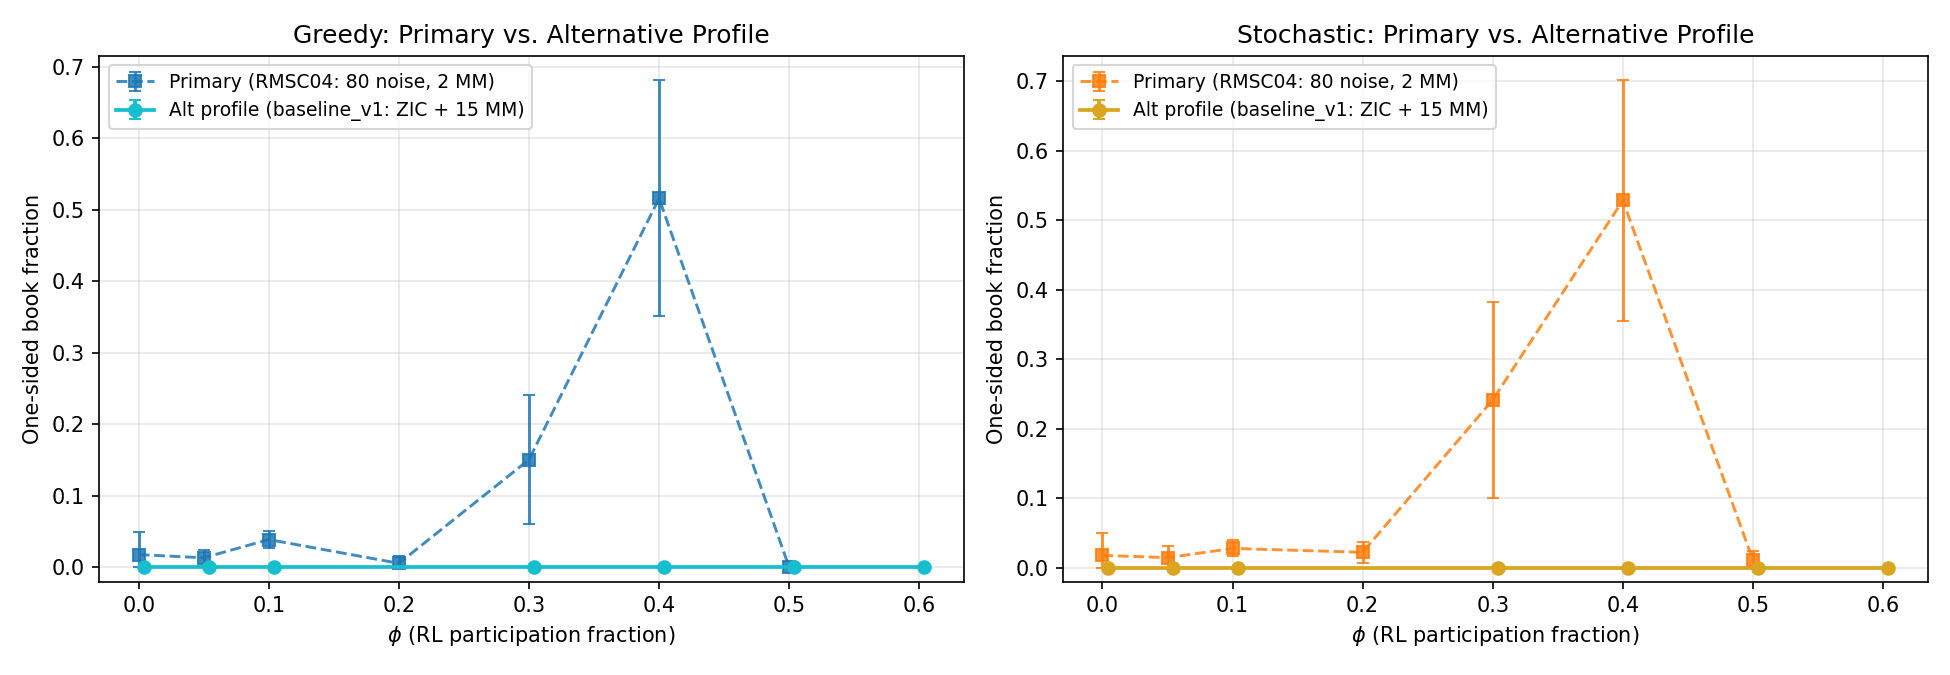
\includegraphics[width=\textwidth]{alt_profile_comparison.png}
    \caption{Robustness check. Under the primary configuration (2 market makers) the failure emerges; under the alternative profile (15 market makers) no one-sided failures are observed at any tested $\phi$ value, consistent with the threshold prediction.}
    \label{fig:alt-profile-comparison}
\end{figure*}

\FloatBarrier

\section{Discussion and Limitations}

The main result is that trained RL agents degrade market structure at the level of top-of-book price formation, not merely through aggregate statistics such as volatility. The failure is mechanistically driven by liquidity imbalance — RL agents consuming faster than background traders replenish — and is distinct from both random participation and market shutdown. The flow-rate model provides a closed-form connection between micro-level agent parameters and the macro-level failure threshold.

Three limitations warrant emphasis. First, the policy is a single linear softmax layer with no hidden layers; a richer architecture may alter both individual behavior and the threshold mechanism. Second, all results are obtained in a single ABIDES-based configuration; the alternative-profile robustness check supports the mechanism, but generalization to other environments requires further study. Third, the training configuration includes hold-streak penalties to discourage degenerate inactivity; different reward specifications could shift the onset $\phi^*$ or eliminate the nonlinear spike. These findings should therefore be interpreted as identifying a reproducible failure mode within this framework rather than a universal property of real markets.

\section{Conclusion}

We show that increasing RL participation fraction $\phi$ in an agent-based market simulation produces a nonlinear rise in persistent one-sided order book states, consistent with a flow-rate threshold predicted at $\phi^* \approx 0.26$. Both trained and random policies produce severe failures above the threshold ($\phi = 0.40$: trained $30.6\%$, random $26.3\%$, overlapping CIs), confirming the effect is structural rather than policy-specific; it is substantially mitigated by inventory constraints. The asymmetric ask-side failure revealed by the missing-side decomposition indicates the failure is driven by a buy-bias in the learned execution strategy, though structural factors also play a role given that random agents produce comparable failures above the threshold. System-level structural effects should therefore be treated as a first-class criterion when designing and evaluating learning-based trading strategies.

\bibliographystyle{ACM-Reference-Format}
\bibliography{references}

\end{document}
